%%%%%%%%%%%%%%%%%%%%%%%%%%%%%%%%%%%%%%%%%
% Thesis 
% LaTeX Template
% Version 1.3 (21/12/12)
%
% This template has been downloaded from:
% http://www.latextemplates.com
%
% Original authors:
% Steven Gunn 
% http://users.ecs.soton.ac.uk/srg/softwaretools/document/templates/
% and
% Sunil Patel
% http://www.sunilpatel.co.uk/thesis-template/
%
% License:
% CC BY-NC-SA 3.0 (http://creativecommons.org/licenses/by-nc-sa/3.0/)
%
% Note:
% Make sure to edit document variables in the Thesis.cls file
%
%%%%%%%%%%%%%%%%%%%%%%%%%%%%%%%%%%%%%%%%%

%----------------------------------------------------------------------------------------
%	PACKAGES AND OTHER DOCUMENT CONFIGURATIONS
%----------------------------------------------------------------------------------------

\documentclass[11pt, a4paper, oneside]{Thesis} % Paper size, default font size and one-sided paper

%\graphicspath{{./Pictures/}} % Specifies the directory where pictures are stored

\usepackage{amsmath}
\usepackage{listings}
\usepackage{color}
\usepackage{todonotes}
\definecolor{dkgreen}{rgb}{0,0.6,0}
\definecolor{gray}{rgb}{0.5,0.5,0.5}
\definecolor{mauve}{rgb}{0.58,0,0.82}

\lstset{frame=tb,
  language=Java,
  aboveskip=3mm,
  belowskip=3mm,
  showstringspaces=false,
  columns=flexible,
  basicstyle={\small\ttfamily},
  numbers=none,
  numberstyle=\tiny\color{black},
  keywordstyle=\color{blue},
  commentstyle=\color{dkgreen},
  identifierstyle=\color{gray},
  stringstyle=\color{mauve},
  breaklines=true,
  breakatwhitespace=true,
  tabsize=3
}

\begin{document}

%----------------------------------------------------------------------------------------
%	TITLE PAGE
%----------------------------------------------------------------------------------------

\begin{titlepage}
\begin{flushleft}
\Large{
\univname\\
\instname\\
\deptname
}
\end{flushleft}
\begin{center}


\vspace{1cm}


\includegraphics[width=0.4\linewidth]{./figures/miskolc_logo}

\vspace{1cm}

{\huge \bfseries \ttitle}\\[0.4cm] % Thesis title

\textsc{\Large \degreename}\\[0.5cm] % Thesis type
 
 \vspace{4cm}

\textit{Készítette:}\\
\authornames\\
\textsc{\authorId}
 
\vspace{2cm}

\textit{Konzulens:}\\
\supname

\vspace{2cm}

\textbf{\the\year.}
%\includegraphics{Logo} % University/department logo - uncomment to place it
 
\vfill
\end{center}

\end{titlepage}

%----------------------------------------------------------------------------------------
%	DECLARATION PAGE
%	Your institution may give you a different text to place here
%----------------------------------------------------------------------------------------

\thispagestyle{empty}
\phantomsection
\addcontentsline{toc}{chapter}{Declaration of Authorship} 
%\null
\vfil
\vskip 60pt
\begin{center}{\huge\bf Declaration of Authorship\par}\end{center}

I hereby certify that this essay has been composed by me and is based on my own work, unless stated otherwise.
No other person's work has been used without due acknowledgement in this essay.
All references and verbatim extracts have been quoted, and all sources of information, including graphs, have been specifically acknowledged.
\paragraph*{}
Miskolc, \today \\

\vspace{2cm}
\begin{minipage}{0.4\textwidth}
\begin{center}
\rule{5cm}{0.5mm} \\
\authornames
\end{center}
\end{minipage}

\clearpage % Start a new pag

\tableofcontents
\newpage

\chapter{Bevezetés}
\label{chapIntroduction}
\paragraph{}
A szoftverfejlesztés a mai világunk egyik alapköve. 
Az informatika világa és a mi hétköznapi eszközeink sem lennének képesek fejlődni a szorgos programozók munkája nélkül. 
Azonban a szoftver fejlesztés nem egy egyszerű dolog, főleg ha egy komplex programozási feladatra van szükség. 
Ilyenkor szinte biztosan nem egy ember fogja elkészíteni ezeket a programokat, így a munka kódolás része kevesebb feladatot ró a fejlesztőre viszont számos egyéb feladattal kell szembe néznie.

\paragraph{}
Ezek a feladatok (ha jól elő vannak készítve) nagyon könnyen vehető akadályok. 
Ha minden új munkatársnak bemutatják hogy milyen struktúrában kell kódolnia vagy vannak egyéb eszközök segítik a munkáját.
Ezek lehetnek verziókövetőrendszerek, automatikus tesztelési környezet vagy akár csak a dokumentum legenerálásában segítő alkalmazás.

A programozókra komoly munka és rengeteg egyeztetés várna, ha nem léteznének úgynevezett verzió követő rendszerek.
Nem is lehetne olyan szoftver gyártó céget mondani mely nem használná valamely formában a Git-et.

Persze ezen felül ha többen dolgoznak egy kódon akkor a csapatmunka gördülékenységét segíti elő bizonyos szabályok lefektetése.
Az ugyan olyan formátumú kód használata elengedhetetlen komplex programok megírásakor.
Vagy a dokumentáció is, hogy a kód később is vagy egy új kolléga számára is egyértelmű legyen.

A Continuous Integration – azaz a folyamatos integráció
---HALO---

A csapatban való munka legalább olyan fontos részét alkotja a modern szoftverfejlesztésnek mint a munkálatokat segítő rendszerek.
Ha egy mai informatikai céget meglátogatunk, azt láthatjuk hogy a programozók nem elszeparáltan hanem egy közös térben dolgoznak.
Például egyre népszerűbb a scrum módszer bevezetése az irodákban és minden reggel ennek megfelelően egy közös megbeszéléssel kezdőik.

A csapatmunkát komoly támogatási háttérrel szükséges ellátni. 
Gondok itt arra, hogy lehetőséget kell adni minden fejlesztő számára, hogy a fejlesztés állapotát nyomon tudják követni és a mások munkáját is könnyen feltudják használni vagy esetenként módosítani tudják azt. 
Ezeket a lehetőségeket nem egy egyszerű feladat megteremteni legyen szó tíz vagy akár százfős irodáról.

\paragraph{}
Ez a téma az informatika nem annyira szembetűnő oldaláról mutatja be. 
A mai világban gyakran hajlamosak vagyunk megfeledkezni arról, hogy az a kép amit elkattintunk a telefonunkkal hogyan is kerül fel a felhőbe és onnan a asztali számítógépünkre vagy akár a barátainkhoz valamilyen közösségi média platform használatának segítségével.
Nem egy program megszületését dokumentáltam hanem sokkal inkább azt, hogy egy komplex programhoz milyen háttér eszközök kellenek hogy elkészüljön.
\pagebreak
\section{Motiváció}
\label{chapMotivation}

\paragraph{}
Mostanra az informatikusnak tanulók között is sokkal izgalmasabb egy mobilfejlesztés vagy egy webfejlesztés.
Az látszik, az van előtérben, végül is az ő munkájuk ami igazán eljut a végfelhasználókhoz.
Ez teljesen megérthető hiszen a színes izgő-mozgó képek tengerével hogyan is vehetné fel a versenyt egy még a Mátrix c. kultuszfilmben is csak keveset látott terminál ablak fekete-zöld karakteri.
Pedig ez a világ az ami lehetővé teszi az eszközök közötti összeköttetést és a csillogó képekkel teli megjelenést.
Az ember azt gondolná hogy a programozók pontosan ismerik ezt a világot, pedig vannak akik ennél is mélyebbre mennek.
Ezek az emberek a rendszerüzemeltetők és az ők titkolt és rejtett világuk.
Pontosan ez tetszett meg nekem és ezért is szeretnék hasonló témában elkészíteni a feladatom.
Természetesen ez talán még nem elég ahhoz hogy egy ilyen témába mélyen beleássa  magát az ember.
Már régebben is az foglalkoztatott hogy bizonyos játékoknak hogyan tudnék saját szervert csinálni hogy a barátainkkal igazán szabadon élvezhessük a játékok adta élményeket.

\paragraph{}
A Miskolci Egyetem Mérnökinformatikai szakán eltöltött éveim során próbáltam a lehető legtöbb olyan sávot választani a tantervi hálóból ami nem fejlesztéssel hanem üzemeltetéssel foglalkozik. 
A fejlesztés sem egy teljesen unalmas ága az informatikának, viszont számomra az üzemeltetés egy sokkal változatosabb világba varázsol el.
A jövő is nagy számítási teljesítmények (Big Data, Deep Learning) felé mutat amelyet nem titkolt célom még a technológia hajnalán elsajátítani. 
Úgy gondolom, hogy a mai fejlesztési feladatinak még nagyobb szüksége van a stabíl, jól működő és állandóan rendelkezésre álló supportra. 
Ezért is ragadtam meg a lehetőséget mikor Dr. Tóth Zsolt konzulensem felajánlott egy projekt munkát a Miskolci Egyetem Informatika Intézetében. 

\paragraph{}
Ez a projekt az ILONA beltéri helymeghatározó rendszernek a fejlesztése során szükségessé vált automatizált tesztelési rendszer és környezet kialakítása volt. 
Mikor elkezdtem foglalkozni a témával még jobban megtetszett az üzemeltetés és a support világa és ekkor gondoltam úgy, hogy ebből szakdolgozatot fogok írni. 
Ezzel a dolgozattal is rengeteg újat dolgot tanultam amit az egyetemi tanórák keretein belül soha sem tanultam volna meg. 

Számomra ez a projekt teljes mértékig szabad kezet adott.
A saját képzeletemnek és ismereteimnek megfelelően tudtam egy teljesen új rendszert megépíteni és mások számára elérhetővé tenni.
Időközben elkezdtem dolgozni is az egyetem mellett ahol ugyan így üzemeltetéssel tudok foglalkozni.
Sok ötletel tudtam eltanulni kollégáimtól és úgy gondolom én is tudtam nekik újat mutatni melyeket itt az egyetemen ezzel a projekttel tanultam meg.


Számomra nagyon fontos volt hogy egy olyan témával tudjak foglalkozni ami maradandó nyomot hagy az egyetemen.
Egy ilyen rendszert felépíteni és üzemeltetni jó lehetőség erre, hiszen a folyamatosan cserélődő fejlesztői csapat sokáig tudja majd használni.
A rendszer úgy van megtervezve hogy bővíthető legyen és esetleges extra igényeket is kitudjon szolgálni a IIT-s csapat számára.

\pagebreak
\section{Célkitűzés}
\label{chapGoal}
\paragraph{}
A célom azt volt, hogy a Miskolci Egyetem Általános Informatika Tanszékén az ILONA rendszeren dolgozó fejlesztőknek a munkáját segítsem. 
A fejlesztők jelenleg az építést és a tesztelést is manuálisan valósítják meg, ahogy ez a \ref{fig:jelenallapot} ábrán is látható. Ez a feladatom kiinduló állapota. 

\begin{figure}[h]
	\centering
	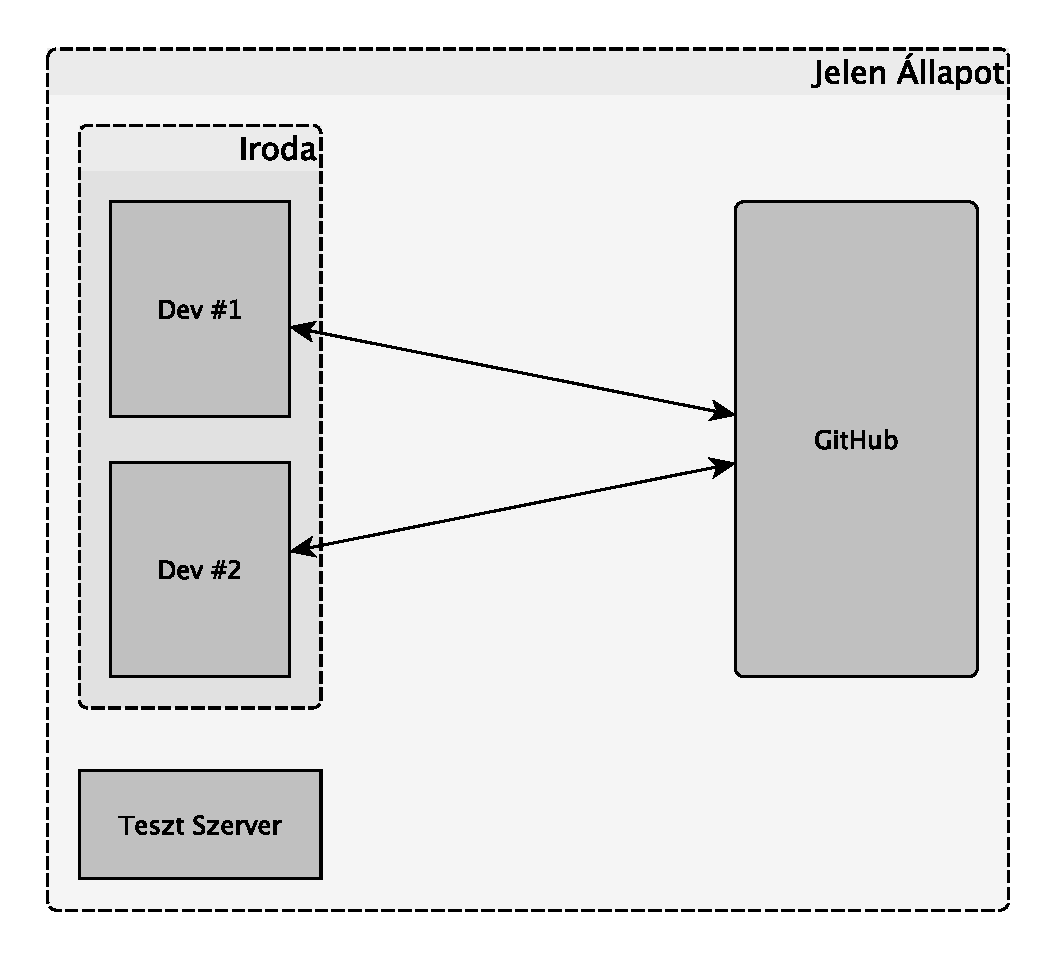
\includegraphics[width=0.7\linewidth]{figures/jelenallapot}
	\caption{Jelen Állapot}
	\label{fig:jelenallapot}
\end{figure}

Az új rendszernek a jelenlegi állapotnak több sajátosságát meg szerettem volna tartani és ezeken felül a már meglévő szerverekkel megvalósítani a rendszer működését. 
Fontosnak tartottam hogy a fejlesztők kizárólag a feladataik csökkenésével szembesüljenek és ne keljen új programokat, folyamatokat megtanulniuk. 
Kvázi ne látszódjon a háttérbe folyó változás és a jelenlegi rendszer szolgáltatás kiesésével se járjon az új rendszer bevezetése. 
Mivel az ILONA fejlesztése teljesen önerőből, támogatás nélkül valósul meg, ezért törekedtem arra hogy csak ingyenes, "opensource" alkalmazásokat használjak a feladathoz. 
Sikerült is ennek eleget tenni, minden komponens opensource és ingyenesen elérhető bárki számára az interneten.

A jelenlegi rendszer alapja az egyik legnépszerűbb ingyenes internetes verziókövető rendszer a GitHub. 
A GitHub-ot feltétlen meg akartam tartani az új rendszerben mivel egy elterjedten használt és kedvelt környezetnek tartom és ami még mellette szól az az ingyenessége. 
Természetesen lehetett volna saját git-et is használni viszont az egyetemi projekteken nem mindig csak a campuson dolgozunk és nem is kell mindig titokban tartani.

A mostani teszt szerver Maven segítségével építi és teszteli a megírt kódokat, ezért a következő amit a meglévő rendszerből át akartam vinni az újba az a Maven. 
A jelenlegi rendszer nem hatékony a munkavégzés során, mivel számos munkaidőt emészt fel a folyamat amely nem a fejlesztéssel kapcsolatos. 

\pagebreak
\paragraph{}
A fejlesztőknek az új rendszerben lényegében csak a GitHubbal és a kész JAR fájlokat tartalmazó repository szerverrel kell dolgozniuk a többi folyamatot automatikusan látná el a rendszer. 
A cél tehát egy olyan Automatikus Tesztelési Környezet megvalósítása, amely képes a GitHubról letölteni a kódokat akkor ha a kódban változás történik. 
Ezen felűl ha a tesztek és a buildelési folyamat is sikeresen végbement az elkészült fájlokat könnyen és szervezetten elérhetővé tennie egy repository szerveren. 
Ez a tervezett folyamat látható a \ref{fig:jovoallapot} ábrán. 


\begin{figure}[h]
	\centering
	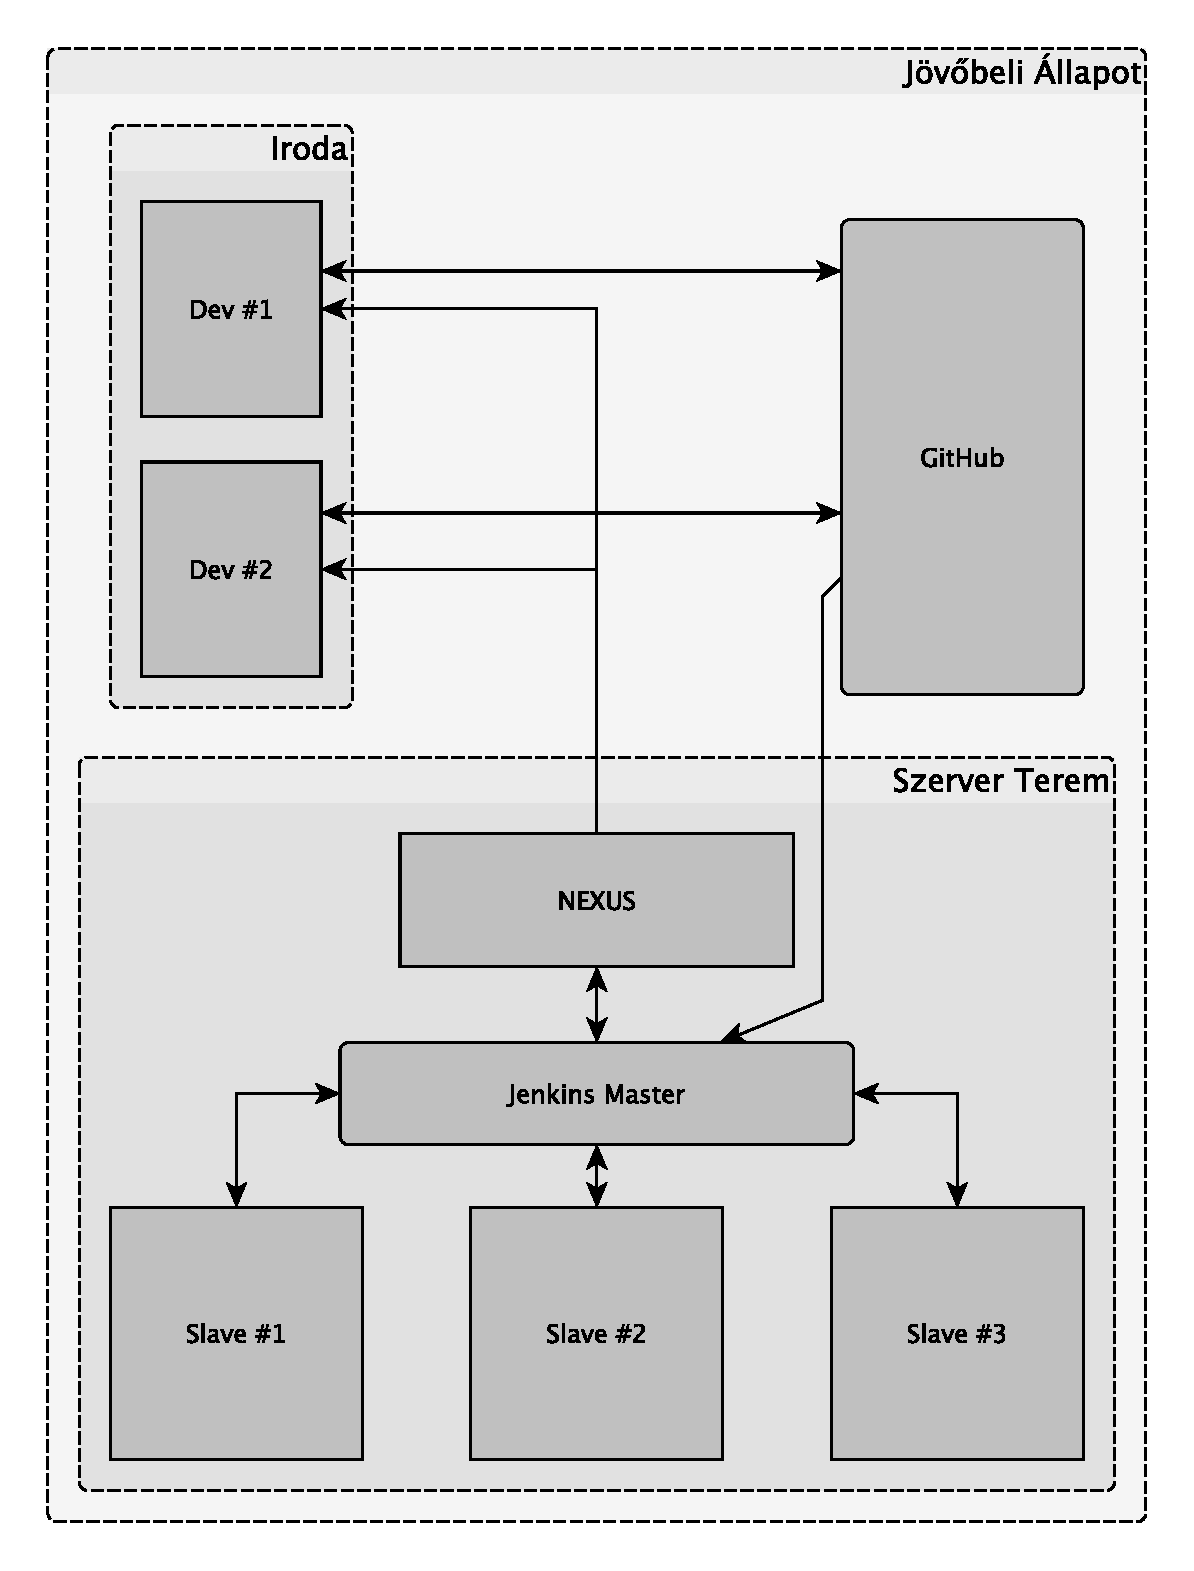
\includegraphics[width=0.7\linewidth]{figures/jovoallapot}
	\caption{Jövő Állapot}
	\label{fig:jovoallapot}
\end{figure}

\chapter{Technológiák}
\label{chapTech}

\section{Docker}
\label{docker}
\paragraph{}
Kezdjük azzal, hogy meghatározzuk, mi a Docker.
Azért a Dockerrel kezdem mivel ez az alapja az egész projektemnek.
A Docker honlapja jelenleg a következőképpen határozza meg a Dockert (Szabad fordításban):

\paragraph{}
"A Docker a világ vezető szoftveres tárolóplatformja, a fejlesztők a Docker-t használják az "én gépemen működik" problémák kiküszöbölése érdekében, amikor a munkatársakkal együtt dolgoznak egy kódon. Az üzemeltetők a Dockert használják az alkalmazások futtatására és kezelésére egy szerveren elválasztva egymástól a legjobb kihasználtságért, A vállalatok a Docker-t használják agilis szoftverszállítási folyamatokhoz, hogy gyorsabbá és biztonságosabbá tegyék a Linux és a Windows Server alkalmazásaikat." \cite{dockerswebpage}

\paragraph{}
Ez egy elég merész megnyitó nyilatkozat, de ha megnézzük a Docker vezérigazgatója, Ben Golub által bemutatott számokat a 2017-es DockerCon megnyitása során, amelyek a következők:

 - 14 millió Docker fogadó
 
 - 900,000 Docker Alkalmazások
 
 - 7700 százalékos növekedés a Docker "Image"-k letöltésében
 
 - 3300 projektpartner

Egy olyan technológia esetében, amely csak három éves, mindenki egyet kell hogy értsen ez meglehetősen lenyűgöző teljesítmény.  \cite{dockercondata2017}

\subsection{Különbségek dedikált hostgépek, vitruális gépek és a Docker közt}
\label{dockerdiff}
A Docker egy konténerkezelő rendszer, amely hasonlít a Linux Containers (LXC)-re de könnyebb és univerzálisabb módon azt.
Lehetővé teszi a virtuális környezetben lévő képek létrehozását akár laptopon, ugyanis a futtatásuk nem igényel nagy erőforrást.
Ebben a környezetben a saját gépén helyi szinten futó konténeren végrehajtott műveletek vagy parancsok ugyanazok amelyeket megszokhattunk egy valódi gépen.
Ez segít abban, hogy ne kelljen másképp csinálni a dolgokat, ha egy olyan fejlesztői környezetből, mint amilyen a helyi gépen található, szerver szintű környezetébe lépünk.

\pagebreak

Nézzük meg a Docker konténerek és egy tipikus virtuális gépi környezet közötti különbségeket.
Az alábbi ábra bemutatja a dedikált, host gép és a virtuális gép közötti különbséget:

\begin{figure}[h]
	\centering
	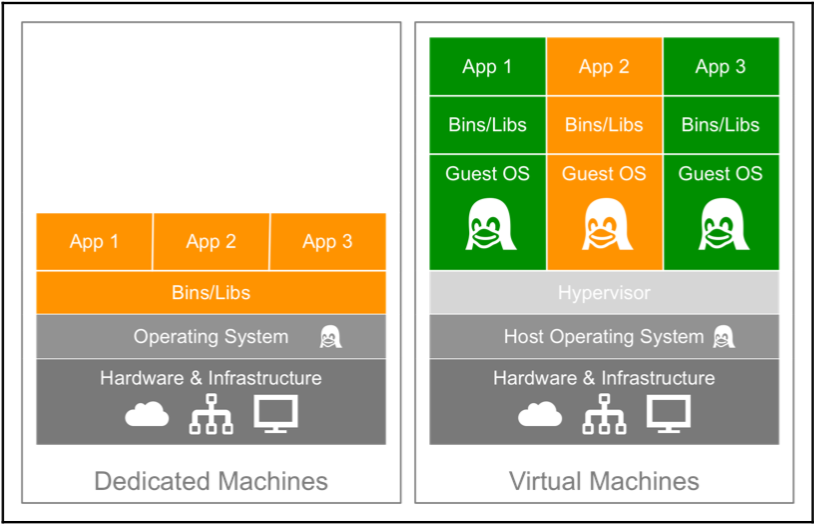
\includegraphics[width=1\linewidth]{figures/host-machine-vs-vm}
	\caption{Egy Host gép és egy Virtuális gép közti különbség}
	\label{fig:hostvsvm}
	\cite{gallagher2015mastering}
\end{figure}

\paragraph{}
Mint látható a kép bal oldalán, egy dedikált gépen három alkalmazást futtatunk, mindegyik ugyanazt a narancssárga szoftvercsomagot tartalmazza. 
Ez egy alap hardver, operációsrendszer, telepített alkalmazások és a hozzájuk tartozó csomagok rendszer.
Nehezen szabályozható, monitorozható és az erőforrás elosztást is nehezen lehet kivitelezni.
A virtuális gépek futtatása már lehetővé teszi számunkra, hogy három alkalmazást futtassunk, két teljesen más szoftvercsomaggal.
Mi szabályozhatjuk hogy a host gépből menyit adunk át a virtuális gépnek és tudjuk őket külön monitorozni.
A kép baloldalán látható hogy a host operációs rendszeren felül még 3 vendég rendszert is futtatnunk kell.
A három rendszer mellett az ábra mutatja ugyanazokat az alkalmazásokat (narancssárga és zöld), amelyek a Docker használatával egy konténerekben futnak, mivel ugyan azokat a csomagokat használják.

\pagebreak

\begin{figure}[h]
	\centering
	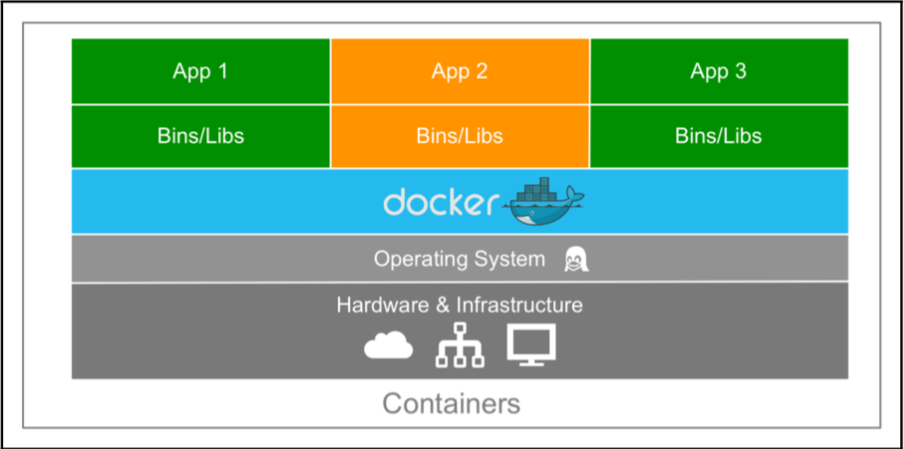
\includegraphics[width=1\linewidth]{figures/docker-work}
	\caption{Egy Dockert futtató gép és konténerei}
	\label{fig:docker-work}
	\cite{gallagher2015mastering}
\end{figure}

\paragraph{}
Ez az illusztráció nagyon jó betekintést nyújt a Docker legfontosabb előnyeibe.
Nincs szükség egy teljes operációs rendszerre minden alkalommal, amikor új konténert hozunk létre ami lecsökkenti a konténerek teljes méretét.
A Docker gazdagép Linux kernelének használatára támaszkodik, mivel a Linux szinte minden verziója a szabványos kernel modelleket használja.
%Így a Docker által épített operációs rendszerek, például a Red Hat, a CentOS és az Ubuntu számára. 
Emiatt szinte bármilyen Linux operációs rendszert futhat a gazda gép, és képes lesz a Linuxon alapuló operációs rendszerek futtatására. 
Ez igaz a Unix alapú operációs rendszerekre is, így egy macOS-el telepített host gép is képes szinte bármilyen Linux konténert futtatni (Kivételek pl.: RHEL, SLES). 
Ugyan az alkalmazások úgy látják hogy egy teljes értékű operációs rendszeren futnak, valójában csak a binálisok és csomagok például Apache, Java és könyvtáraik szükségesek az alkalmazások futtatásához.
Például a korábbi ábrán látható, hogy például a narancssárga alkalmazáshoz Red Hat, a zöld alkalmazáshoz pedig Debian szükséges.
Soha nem lesz szükség a Red Hat vagy a Debian telepítésére, így a Docker egy másik előnye a képek mérete kerül előtérbe.
A konténerek a legnagyobb darab nélkül épülnek fel azaz a rendszermag vagy az operációs rendszer nélkül.
Így rendkívül kicsi, kompakt és könnyen szállítható "konténereket" kapunk.


\pagebreak
\subsection{Maven}
\paragraph{}
Az Apache Maven népszerű, mint építési eszköz. Rövid nevén csak Maven-t szoftverfejlesztés során használjuk a projektek menedzselésére. 
A valóságban azonban túlmutat azon, hogy ez csak egy "build" eszköz.
Átfogó "build"-elési menedzsment platformot biztosít.
\paragraph{}
A Maven történe.
A fejlesztőknek sok időt kellett tölteniük egy építési rendszer kiépítésében. Nem volt közös felület.
Ez minden projektnék különbözött. Olyan esetben, amikor egy fejlesztő egyik projektről a másikra költözött, újra meg kellett a buildelést tanulnia.
Maven betöltötte ezt a rést egy közös felület bevezetésével. Ez véget vetett az "építőmérnök" korának.
\paragraph{}
Az Apache Ant utódja, sok tekintetben hasonlít a két szoftver, azonban az Ant lassabb és elavultabb mint a Maven. 
A Mavennel az építési- és tesztelési folyamatok automatizálhatóak, így a Jenkinsel tökéletesen együtt tud dolgozni. 
A Maven egy új fogalmat is bevezet, ez az úgynevezett Projekt Objektummodell (angolul: Project Object Modell) röviden a POM. 
A POM egy XML fájl amely egy építésre kész projektet és annak függőségeit írja le. 
Ezzel a pom.xml fájllal adjuk meg a Mavennek hogy mit is csináljon a kóddal.
Előre megadott célokat tartalmaz mint a kód fordítása és csomagolása, azonban itt van lehetősége a fejlesztőknek saját célokat és teszteket létrehozni. 

\paragraph{}
A Mavent 2002-ben Jason van Zyl készítette el. A projektet az Apache Software Foundation fejleszti, korábban a cégnél a Jakarta Projekt részeként működött. Jelenleg a 3.3.9-es a legfrissebb verziója.

\paragraph{}
A Maven hálózatképes, tehát szükség esetén dinamikusan is le tud tölteni komponenseket.
Repository névvel illetik a különböző hosztok fájlrendszereinek azon mappáit, ahol a letölthető komponensek találhatók.
A Maven nem csak a repository-kból való letöltést támogatja, hanem a készült szoftvercsomag feltöltését is. 
Ezzel az automatizálható le- és feltöltési mechanizmussal a Maven de facto szabványt próbál teremteni, de elég lassan fogadja el a Java közösség.
A Maven plugin alapú architektúrája lehetővé teszi tetszőleges parancssorból vezérelhető alkalmazás használatát. 
Ez elméletileg lehetővé teszi tetszőleges programnyelvekhez való pluginek készítését, de a gyakorlatban minimális mennyiségű nem javás plugin készült.

\paragraph{}
A Projekt Objektummodell fontos részét képezi a Mavennek ezért kell róla beszélnünk.
Ahogy azt már beszéltük minden Maven projekt tartalmaz egy pom.xml fájlt.
A pom.xml fájl a projekt XML-ábrázolása, és így tartalmazza a projekthez tartozó összes metaadatot.
Ez magában foglalja a projektkonfigurációt, a hibakövető rendszer részleteit, az engedélyeket, a projektútvonalakat, a függőségeket stb.
A POM definíciónak tartalmaznia kell legalább három mezőt, ezek a groupId, a artifactId és a verzió.
\pagebreak

\paragraph{}
Ez egy alap pom.xml tartalma:
\begin{lstlisting}
	<project ... >
	<modelVersion>4.0.0</modelVersion>
	<!-- The Basics -->
	<groupId>...</groupId>
	<artifactId>...</artifactId>
	<version>...</version>
	<packaging>...</packaging>
	<dependencies>...</dependencies>
	<parent>...</parent>
	<dependencyManagement>...</dependencyManagement>
	<modules>...</modules>
	<properties>...</properties>
	<!-- Build Settings -->
	<build>...</build>
	<reporting>...</reporting>
	<!-- Project Meta Data -->
	<name>...</name>
	<description>...</description>
	<url>...</url>
	<inceptionYear>...</inceptionYear>
	<licenses>...</licenses>
	<organization>...</organization>
	<developers>...</developers>
	<contributors>...</contributors>
	<!-- Environment -->
	<issueManagement>...</issueManagement>
	<ciManagement>...</ciManagement>
	<mailingLists>...</mailingLists>
	<scm>...</scm>
	<prerequisites>...</prerequisites>
	<repositories>...</repositories>
	<pluginRepositories>...</pluginRepositories>
	<distributionManagement>...</distributionManagement>
	<profiles>...</profiles>
	</project>
\end{lstlisting}

A bemutatott POM minta négy fő részből áll. Ezek a következők:

\paragraph{Az alapok:} Ez a rész a projekt koordinátáit, a függőségkezelést és az örökség részleteit tartalmazza.
Ezenkívül modulokat és projektszintű tulajdonságokat is tartalmaz.
\paragraph{Build beállítások:} Ez a rész tartalmazza a részleteket.
\paragraph{Projekt metaadatai:} Ez a szakasz olyan projekt-specifikus adatokat tartalmaz, mint a név,
szervezet, fejlesztők, URL, kezdési év stb.
\paragraph{Környezet:} Ez a rész a környezetre vonatkozó összes információt tartalmazza, beleértve a verziókezelés részleteit, a kiadáskezelést, a folyamatos integrációt, a levelezőlistákat, a tárolókat stb.

\pagebreak

\subsection{Java, JUnit}

\subsubsection{Java}
\paragraph{}
---IDÉZERT---
A Java általános célú, objektumorientált programozási nyelv, amelyet a Sun Microsystems fejlesztett a ’90-es évek elejétől kezdve egészen 2009-ig, amikor a céget felvásárolta az Oracle. 2011-ben a Java 1.7-es verzióját az új tulajdonos gondozásában adták ki.

A Java alkalmazásokat jellemzően bájtkód formátumra alakítják, de közvetlenül natív (gépi) kód is készíthető Java forráskódból. A bájtkód futtatása a Java virtuális géppel történik, ami vagy interpretálja a bájtkódot, vagy natív gépi kódot készít belőle, és azt futtatja az adott operációs rendszeren. Létezik közvetlenül Java bájtkódot futtató hardver is, az úgynevezett Java processzor.

A Java nyelv a szintaxisát főleg a C és a C++ nyelvektől örökölte, viszont sokkal egyszerűbb objektummodellel rendelkezik, mint a C++. A JavaScript szintaxisa és neve hasonló ugyan a Java-éhoz, de a két nyelv nem áll olyan szoros rokonságban, mint azt ezekből a hasonlóságokból gondolhatnánk.

Bár a nyelv neve kezdetben Oak (tölgyfa) volt, (James Gosling, a nyelv atyja nevezte így az irodája előtt növő tölgyfáról), később kiderült, hogy ilyen elnevezésű nyelv már létezik, ezért végül Java néven vált ismertté. A Java szó a Oracle védjegye. Ennélfogva engedélye nélkül nem használható mások által kifejlesztett termékek megjelölésére; még például Java-szerű ... stb. összetételben sem, mert ez a védjegyjogosult jogaiba ütközik.
---IDÉZERT---

\subsubsection{JUnit}
---IDÉZERT---
JUnit egy egységteszt keretrendszer Java programozási nyelvhez. A teszt vezérelt fejlesztés (TDD) szabályai szerint ez annyit tesz, hogy a kód írásával párhuzamosan fejlesztjük a kódot tesztelő osztályokat is (ezek az egység tesztek). Ezeken egységtesztek karbantartására, csoportos futtatására szolgál ez a keretrendszer. A JUnit teszteket gyakran a build folyamat részeként szokták beépíteni. Pl. napi build-ek esetén ezek a tesztek is lefutnak. A release akkor hibátlan, ha az összes teszt hibátlanul lefut.

A JUnit a egységteszt keretrendszerek családjába tartozik, melyet összességében xUnit-nak hívunk, amely eredeztethető a SUnitból.

JUnit keretrendszer fizikailag egy JAR fájlba van csomagolva. A keretrendszer osztályai következő csomag alatt található:

JUnit 3.8-as ill. korábbi verzióiban a junit.framework alatt találhatók
JUnit 4-es ill. későbbi verzióiban org.junit alatt találhatók
---IDÉZERT---

\paragraph{}
Az ILONA rendszer a fejlesztők Java nyelven fejlesztik, ezért az új rendszernek képesnek kellett lennie a Java használatára. 
Emellett maga a Jenikins CI is egy Java nyelven íródott webalkalmazás ami Java VM-en fut. 
Így a Safranek virtuális gépre egy legfrissebb Java 

\subsection{Jenkins}
A Jenkins egy nyílt forráskódú, Java nyelven írott eszköz amely folyamatos integrációs szolgáltatást nyújt szoftverfejlesztéshez. 
Az Oracle Hudson folyamatos integrációs eszközének eredeti fejlesztő csapata vált ki a Hudson fejlesztéséből és valósították meg a Jenkinst. 
Mivel az eredeti fejlesztőcsapat jelenleg is a Jenkinst fejleszti ezért érdemes (ha a kettő közül kell választanunk) a Jenkinst választani. 
A Jenkins mellet szóló érv még hogy több plugin érhető el hozzá mint a Hudsonhoz, így több feladatot is egyszerűbben valósítható meg. 
Ezt az eszköz közvetlenül telepíthetjük a rendszerünkre, viszont választhatjuk hogy egy szervlet konténerben fusson, mint pl. az Apache Tomcat. 
Támogat számos SCM eszközt mint például a Git-et amely az ILONA projekt számára elengedhetetlen. 
Ezek mellett az Apache Ant és Apache Maven parancait is végre tudja hajtani, így a Maven továbbra is lehetséges használni az új rendszerben. 
A Jenkins elsődleges fejlesztője Kohsuke Kawaguchi. A Jenkinst MIT licenc alatt adják ki és szabad szoftver. 

“A Continuous Integration – azaz a folyamatos integráció – egy szoftver fejlesztési módszer melyben a fejlesztőcsapat tagjai az általuk írt kódot legalább napi rendszerességgel integrálják a korábbi fejlesztések közé, ez napi többszöri integrálást jelent. Minden új kód integrálása során automatizált tesztek ellenőrzik, hogy a rendszerbe való illesztés során okozott-e valamilyen hibát az új kódrészlet és ennek eredményeként a lehető leghamarabb visszajelzést ad az integráció eredményéről”
\cite{fowler2006continuous}

Maga a Jenkins CI látja egy a különböző elemek közti kapcsolatot, a GutHub hookjaitól egészen a Maven építési és tesztelési folyamat visszajelzéséig. 

\subsection{Nexus}

---IDE MÉG NEM TALÁLTAM SEMMIT, DE MAJD TALÁLOK KI---

\chapter{Tervezés}
\label{chapTerveres}

Lemásolni a miskolci cégek jelenleg használt technológiák fejlesztési környezetek labor környezetben való kiépítése.

\section{Honnan hova jutunk}

Az eredetei állapot alapjait amelyet a \ref{fig:jelenallapot} ábrán láthatunk, teljesen megtartásra kerülnének. 
Ez a GutHub mint verziókövető rendszer és a Maven mint tesztelésre használt program. 
Minden szempontot figyelembe véve a \ref{fig:jovoallapot} ábrán látható rendszer megvalósítása a 

\section{Hogyan?}


\section{Formális leírás}

Táblázat
milyen gép, gépek igényei és elérhetőségei

migrálható komponensek

\section{Lépések (logikailag)}

\subsection{Szerverek}
A rendszer megépítésekor már meglévő eszközök megtartásra kerülnek. 
Ezért az első feladat a Safranek virtuális szervergép frissítése és a szükséges függőségek telepítése. 
Ezen felül mivel a Jenkinst egy Tomcat fogja futtatni, ezért a Tomcat legújabb verziójának a telepítését kell megoldanunk. 


---JENKINS SZERVER---

---JENKINS SZERVER ÉS A SLAVEK---

---JENKINS SZERVER ÉS A GITHUB---

---GITHUB ÉS A FEJELSZTŐK---

---JENKINS SZERVER ÉS A NEXUS SZERVER---

---NEXUS SZERVER ÉS A FEJLESZTŐK---

---EGYBE A MŰKÖSÉS---


---JENKINS SZERVER---

A fő Jenkins szervernek nincs nagy erőforrás igénye, viszont nagy tárhelykapacitással kell rendelkeznie és könnyen elérhetőnek kell lennie. Ezért a tanszéken meglévő safranek nevű virtuális szerverre esett a választásom mivel ez a szerver nem csak a belsőhálózatból elérhető és dinamikusan növelhető tárhely kapacitással rendelkezik. Ennek a szervernek lényegében csak egy TomCat-ot és magát a Jenkins kell futtatnia számítások elvégzése nélkűl.

---JENKINS SZERVER ÉS A SLAVEK---

Fontos volt a projekt megvalósítása során, hogy a rendszer könnyen bővíthető legyen és több platformra is képes legyen buildeli és tesztelni. Ezért Master-Slave rendszerel terveztem megvalósítani a Jenkins CI-t. Ugyanis egy Jenkns Master szerver is képes több platformara tesztelni és buildelni, ha legalább egy Slave szerveren megtalálhatóak az adott platformhoz szükséges csomagok és függőségek. Első sorban azokat az igényeket kellett felmérni a jelenlegi és jövőbeli feladatok problémamentes kiszolgálása érdekében az indulásnál már meg kell lenniük---LEHET EZ IS HÜLYESÉG---.

---JENKINS SZERVER ÉS A GITHUB---

A következő lényeges feladat az automatikus GitHub pull-olás beállítása volt. Itt a lehető legnagyobb biztonság elérése és az automatizáltság miatt ssh kulcsos azonosítást szerettem volna megvalósítani. Így a fejlesztőknek a kódoláson kívül csak a GitHub-ra való szinkronizálás lenne a feladatuk.
\chapter{Implementáció}
\label{chapImplemetacio}

%Install ubuntu server
%Install docker
%https://docs.docker.com/install/linux/docker-ce/ubuntu/
%Install docker registry
%Install docker registry web interface
%https://hub.docker.com/r/hyper/docker-registry-web/
%Install Jekins docker
%https://hub.docker.com/r/jenkins/jenkins/
%Install Jenkins docker plugin
%Docker Slaves plugin
\section{Szerverek}

\subsubsection{Safranek}

\paragraph{}
A feladatok közül a legelső a már meglévő Safranek szerver frissítése és konfigurálása volt. 
A Safraneken egy Ubuntu server 16.04-es verzió futott, így nem volt szükség sem az operációs rendszer, sem pedig a disztribúció cseréjére, mivel a projektet az Ubuntu szerver ezen verziója tökéletesen kiszolgálja.
A frissítéseket követően, a Jenkins CI futtatását kellett előkészíteni. 
Egy jenkins nevű felhasználót kellett létrehozni, hogy szeparáltan lehessen futtatni a programokat és az autentikáció során ne a root felhasználó adatait keljen felhasználni. 

Mivel a TomCat és a Jenkins is egy-egy java alapú alkalmazás ezért a Java JRE és JDK legfrissebb verzióját kellett felkellet telepíteni. 
Azt a következő két parancs alkalmazásával: 

----"sudo apt-get install default-jre \&\& sudo apt-get install default-jdk"------


\paragraph{}
Az első felhasználó létrehozásához és a komponensek telepítése előtt egy a "/.jenkins/secrets/initialAdminPassword" fájlban található jelszót kell bemásolni a formba a folytatáshoz. 
Miután ez megtörtént a Jenkins CI admin felülete tárul elénk \ref{fig:clearjenkins}. 

\subparagraph{Jenkins}

A Jenkin CI 
\chapter{Tesztelés}
\label{chapTeszteles}
\chapter{Összefoglalás}

asdf \cite{berg2012jenkins}


\bibliographystyle{plain}
\bibliography{references}

\appendix

%\chapter{CD Melléklet}

Lorem ipsum dolor sit amet, consectetuer adipiscing elit, sed diam nonummy nibh euismod tincidunt ut laoreet dolore magna aliquam erat volutpat. Ut wisi enim ad minim veniam, quis nostrud exerci tation ullamcorper suscipit lobortis nisl ut aliquip ex ea commodo consequat. Duis autem vel eum iriure dolor in hendrerit in vulputate velit esse molestie consequat, vel illum dolore eu feugiat nulla facilisis at vero eros et accumsan et iusto odio dignissim qui blandit praesent luptatum zzril delenit augue duis dolore te feugait nulla facilisi. Nam liber tempor cum soluta nobis eleifend option congue nihil imperdiet doming id quod mazim placerat facer possim assum. Typi non habent claritatem insitam; est usus legentis in iis qui facit eorum claritatem. Investigationes demonstraverunt lectores legere me lius quod ii legunt saepius. Claritas est etiam processus dynamicus, qui sequitur mutationem consuetudium lectorum. Mirum est notare quam littera gothica, quam nunc putamus parum claram, anteposuerit litterarum formas humanitatis per seacula quarta decima et quinta decima. Eodem modo typi, qui nunc nobis videntur parum clari, fiant sollemnes in futurum.

\end{document}